\chapter{Landau--Vishkin}

\scan{48}
L'algoritmo di \textbf{Landau--Vishkin} è un esempio di \emph{programmazione
dinamica ibrida}: mescola la tabella di programmazione dinamica
dell'allineamento con le strutture dati per stringhe (i suffix tree), e arriva a
\[
  \Oh(m+n)
\]
per risolvere l'allineamento a distanza $\le k$, purché $k$ sia
\emph{costante}. Nella notazione asintotica restano infatti nascoste delle
costanti, e una di esse è proprio $k$: il costo effettivo è
$\Oh\bigl(k\,(m+n)\bigr)$, che diventa lineare solo perché $k=\Oh(1)$.

Come di consueto $T$ è il testo e $P$ è il pattern, con $m=\abs{T}$ e
$n=\abs{P}$, e nelle applicazioni $\abs{P}\ll\abs{T}$. Il problema che vogliamo
risolvere è il \emph{matching con al più $k$ differenze}: individuare tutte le
posizioni di $T$ in cui termina un'occorrenza di $P$ a distanza di edit al
più $k$.

\begin{figure}[H]
  \centering
  % lv-testo-pattern -- il testo T (lungo) e il pattern P (corto), con |P| << |T|
% (quaderno, pag. 48).  Le graffe con m ed n non sono nel manoscritto: servono a
% fissare la notazione usata subito prima nel testo.
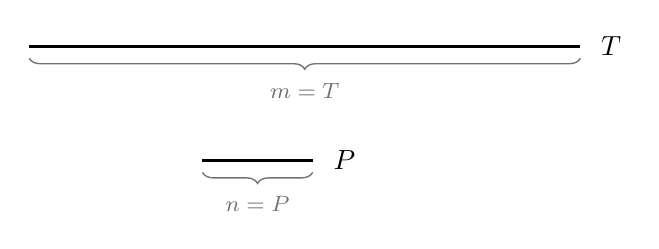
\begin{tikzpicture}[font=\footnotesize]

  % --- il testo ---
  \draw[line width=1.1pt] (0,1.45) -- (7,1.45);
  \node[right=4pt,font=\normalsize] at (7,1.45) {$T$};
  \draw[decorate,decoration={brace,mirror,amplitude=4pt},draw=black!55,
        line width=0.5pt] (0,1.30) -- (7,1.30);
  \node[text=black!55] at (3.5,0.88) {$m=\abs{T}$};

  % --- il pattern ---
  \draw[line width=1.1pt] (2.2,0) -- (3.6,0);
  \node[right=4pt,font=\normalsize] at (3.6,0) {$P$};
  \draw[decorate,decoration={brace,mirror,amplitude=4pt},draw=black!55,
        line width=0.5pt] (2.2,-0.15) -- (3.6,-0.15);
  \node[text=black!55] at (2.9,-0.55) {$n=\abs{P}$};

\end{tikzpicture}

  \caption{Il testo $T$ e il pattern $P$: si cercano le occorrenze di $P$ in $T$
  a distanza di edit $\le k$.}
  \label{fig:lv-testo-pattern}
\end{figure}

\section{L'idea: restare dentro una banda di diagonali}

La tabella di programmazione dinamica ha quindi $n+1$ righe (indicizzate dai
caratteri di $P$) e $m+1$ colonne (indicizzate dai caratteri di $T$). Se
guardassi tutta la matrice il costo sarebbe $\Oh(m\cdot n)$: l'idea è invece di
non uscire mai da una \emph{banda} di diagonali.

\begin{figure}[H]
  \centering
  % lv-banda-diagonali -- la tabella di programmazione dinamica (n+1 righe, m+1
% colonne, con m >> n: rettangolo largo e basso) e la banda di 2k+1 diagonali
% attorno alla diagonale di riferimento (quaderno, pag. 48).
\begin{tikzpicture}[
    font=\footnotesize,
    bordo/.style={line width=0.9pt, line join=round},
    onda/.style={draw=black!70, line width=0.6pt},
    diag/.style={line width=1.4pt, line cap=round},
    fre/.style={line width=0.6pt, -{Stealth[length=2.2mm,width=1.7mm]}},
  ]

  \def\Hh{2.6}

  % --- bordo della tabella: le righe sono indicizzate da P, le colonne da T ---
  \draw[bordo] (0,0) rectangle (11,\Hh);
  \node[left=4pt,font=\normalsize]  at (0,1.30)     {$P$};
  \node[above=3pt,font=\normalsize] at (10.75,\Hh) {$T$};

  % --- le due curve che delimitano la banda -------------------------------
  \draw[onda] plot[domain=0:1,samples=80,smooth,variable=\x]
      ({3.0+2.3*\x+0.13*sin(720*\x)},{\Hh*(1-\x)});
  \draw[onda] plot[domain=0:1,samples=80,smooth,variable=\x]
      ({5.8+2.3*\x+0.13*sin(720*\x)},{\Hh*(1-\x)});

  % --- la diagonale di riferimento: il tratto di match "gratis" -----------
  \draw[diag] (4.4,\Hh) -- (6.7,0);

  % --- scostamento massimo dalla diagonale --------------------------------
  \coordinate (C) at (5.55,1.30);
  \draw[fre] (C) -- (5.55,2.30);
  \draw[fre] (C) -- (5.55,0.32);
  \draw[fre] (C) -- (4.28,1.30);
  \draw[fre] (C) -- (6.82,1.30);
  \node at (5.88,0.55) {$k$};

\end{tikzpicture}

  \caption{La banda di diagonali. Il cammino di allineamento parte lungo una
  diagonale e, avendo a disposizione $k$ errori, può scostarsene di al più $k$
  posizioni in ciascuna direzione: resta perciò confinato fra le due curve che
  delimitano la banda.}
  \label{fig:lv-banda-diagonali}
\end{figure}

Ogni mossa non diagonale --- orizzontale (spazio in $P$) o verticale (spazio in
$T$) --- sposta il cammino di esattamente una diagonale, mentre le mosse
diagonali, di match o di sostituzione, lasciano invariato il numero di
diagonale. Disponendo di al più $k$ errori, il cammino resta dunque confinato in
una banda di $2k+1$ diagonali attorno a quella di partenza, e il lavoro
complessivo scende da $\Th(m\cdot n)$ a $\Oh\bigl(k\,(m+n)\bigr)$.

Restano però da attraversare rapidamente i lunghi tratti di \emph{match} lungo
una stessa diagonale: è esattamente a questo che serve l'intermezzo seguente.

\section{Intermezzo: longest common extension}

È uno dei \emph{by-product} del suffix tree.

\begin{definizione}[Longest common extension]
\label{def:lce}
  Siano $S_1$ e $S_2$ due stringhe e siano
  \[
    i\in\set{1,\dots,\abs{S_1}}, \qquad j\in\set{1,\dots,\abs{S_2}}.
  \]
  Dati $S_1$, $S_2$, $i$ e $j$, si cerca il massimo $k$ tale che
  \[
    \sub{S_1}{i}{i+k-1} \;=\; \sub{S_2}{j}{j+k-1},
  \]
  cioè la lunghezza del più lungo prefisso comune dei due suffissi
  $\suf{S_1}{i}$ e $\suf{S_2}{j}$. La indicheremo con $\lcey(S_1,S_2,i,j)$.
\end{definizione}

\begin{osservazione}
  Il $k$ della definizione di longest common extension è un semplice riuso del
  nome: non ha nulla a che vedere con il numero $k$ di errori ammessi
  nell'allineamento.
\end{osservazione}

Lo strumento per rispondere è il suffix tree generalizzato delle due stringhe,
concatenate per mezzo di due terminatori distinti:
\[
  \STree\bigl(S_1\,\text{\$}\,S_2\,\text{\texteuro}\bigr),
\]
la cui costruzione richiede tempo lineare.

\begin{figure}[H]
  \centering
  % lv-stree-lce -- lo STree generalizzato di S_1 $ S_2 € visto come triangolo:
% la stringa beta letta dalla radice a un nodo interno v e' l'estensione comune
% ai due suffissi che scendono dai rami sotto v (quaderno, pag. 48).
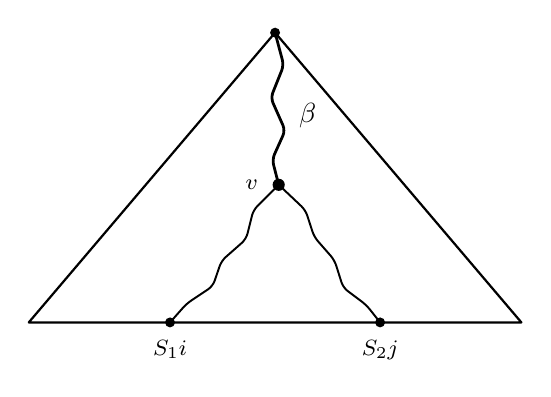
\begin{tikzpicture}[
    x=0.92cm, y=0.92cm,
    font=\footnotesize,
    nodo/.style={circle,fill=black,inner sep=0pt,minimum size=3.6pt},
    ramo/.style={line width=0.7pt, rounded corners=2pt, line join=round},
  ]

  %% ---- la sagoma dell'albero ---------------------------------------
  \coordinate (R) at (0,4);
  \draw[line width=0.8pt, line join=round] (-3.4,0) -- (R) -- (3.4,0) -- cycle;

  %% ---- il cammino radice -> v, etichettato beta ---------------------
  \node[nodo] at (R) {};
  \draw[ramo,line width=1.0pt]
      (0,4) -- (0.12,3.55) -- (-0.06,3.10) -- (0.14,2.65) -- (-0.04,2.25)
           -- (0.05,1.90);
  \node[font=\normalsize] at (0.45,2.85) {$\beta$};

  \node[nodo,minimum size=4.4pt] (v) at (0.05,1.90) {};
  \node[left=4pt] at (v) {$v$};

  %% ---- i due rami che scendono da v ---------------------------------
  \draw[ramo]
      (0.05,1.90) -- (-0.30,1.55) -- (-0.40,1.15) -- (-0.74,0.85)
                  -- (-0.86,0.50) -- (-1.22,0.26) -- (-1.45,0);
  \draw[ramo]
      (0.05,1.90) -- ( 0.42,1.55) -- ( 0.54,1.18) -- ( 0.82,0.86)
                  -- ( 0.94,0.48) -- ( 1.26,0.24) -- ( 1.45,0);

  \node[nodo] (fi) at (-1.45,0) {};
  \node[nodo] (fj) at ( 1.45,0) {};
  \node[below=3pt] at (fi) {$\suf{S_1}{i}$};
  \node[below=3pt] at (fj) {$\suf{S_2}{j}$};

\end{tikzpicture}

  \caption{Nello \STree di $S_1\,\text{\$}\,S_2\,\text{\texteuro}$, la stringa
  $\beta$ letta dalla radice fino a un nodo interno è l'estensione comune ai due
  suffissi che scendono dai due rami sottostanti.}
  \label{fig:lv-stree-lce}
\end{figure}

Ogni nodo dell'albero corrisponde infatti alla stringa $\beta$ che si legge
lungo il cammino dalla radice al nodo, e ogni tale $\beta$ è un \emph{prefisso
di un suffisso} di $S_1\,\text{\$}\,S_2\,\text{\texteuro}$. Posso allora
etichettare l'albero indicando quali di questi prefissi di suffissi occorrono
sia in $S_1$ sia in $S_2$: sono esattamente i candidati a essere estensioni
comuni alle due stringhe.

\scan{49}
In definitiva, la longest common extension si risolve in tempo lineare
procedendo in tre passi.

\begin{enumerate}
  \item Si costruisce il suffix tree generalizzato
        $\STree\bigl(S_1\,\text{\$}\,S_2\,\text{\texteuro}\bigr)$: usando i due
        terminatori distinti \$ e \texteuro{} ogni suffisso è associato a una
        foglia (nessun suffisso è prefisso proprio di un altro, quindi la
        corrispondenza fra suffissi e foglie è biunivoca).
  \item Con una visita \emph{bottom-up} si identificano i nodi che corrispondono
        a prefissi di suffissi sia di $S_1$ sia di $S_2$; nella stessa visita si
        calcolano le profondità in caratteri di tutti i nodi.
  \item Il valore cercato è la profondità massima di un nodo identificato da $i$
        e da $j$: è cioè la profondità, misurata in caratteri, del più profondo
        antenato comune delle due foglie corrispondenti.
\end{enumerate}

\begin{osservazione}
  I primi due passi sono un preprocessing lineare, da eseguire una volta sola.
  Aggiungendovi il preprocessing per le query di $\lca$ su
  $\STree\bigl(S_1\,\text{\$}\,S_2\,\text{\texteuro}\bigr)$ --- anch'esso
  lineare, per Harel--Tarjan --- il terzo passo diventa una singola query di
  $\lca$: si risponde quindi a $\lcey(S_1,S_2,i,j)$ in tempo $\Oh(1)$.
\end{osservazione}

\begin{figure}[H]
  \centering
  % lce-lca -- la query lce(S_1,S_2,i,j) si riduce a una query di lca sullo STree
% generalizzato di S_1 $ S_2 €: le posizioni i e j individuano due foglie, e la
% profondita' in caratteri del loro lca vale k (quaderno, pag. 49).
\begin{tikzpicture}[
    font=\footnotesize,
    nodo/.style={circle,fill=black,inner sep=0pt,minimum size=3.4pt},
    ramo/.style={line width=0.7pt, rounded corners=2pt, line join=round},
    link/.style={draw=black!65, line width=0.6pt,
                 -{Stealth[length=2.2mm,width=1.7mm]}},
  ]

  %% ================= la stringa concatenata =========================
  \draw[line width=0.7pt] (0,4.20) rectangle (6.20,4.75);
  \draw[draw=black!45,line width=0.4pt] (2.90,4.20) -- (2.90,4.75);
  \node[above=2pt] at (3.10,4.75) {$S_1\,\text{\$}\,S_2\,\text{\texteuro}$};

  % le due posizioni interrogate
  \draw[line width=0.6pt,-{Stealth[length=2mm,width=1.6mm]}]
        (1.86,3.92) -- (1.86,4.17);
  \draw[line width=0.6pt,-{Stealth[length=2mm,width=1.6mm]}]
        (3.41,3.92) -- (3.41,4.17);
  \node[font=\normalsize] at (1.86,3.68) {$i$};
  \node[font=\normalsize] at (3.41,3.68) {$j$};

  %% ================= lo STree generalizzato =========================
  \coordinate (R)  at (9.10,4.90);
  \coordinate (bl) at (7.40,1.30);
  \coordinate (br) at (11.00,1.30);
  \draw[line width=0.8pt,line join=round] (bl) -- (R) -- (br) -- cycle;
  \node[nodo] at (R) {};

  % cammino radice -> v e sua profondita' in caratteri
  \draw[ramo,line width=1.0pt]
      (9.10,4.90) -- (9.18,4.62) -- (9.00,4.35) -- (9.14,4.14) -- (9.05,3.95);
  \node[nodo,minimum size=4.4pt] (v) at (9.05,3.95) {};
  \node at (7.72,4.24) {$v=\lca$};
  \draw[draw=black!55,line width=0.4pt] (8.40,4.19) -- (8.96,4.00);

  % la profondita' in caratteri di v: e' il k cercato
  \draw[draw=black!45,line width=0.35pt,dotted] (9.10,4.90) -- (10.42,4.90);
  \draw[draw=black!45,line width=0.35pt,dotted] (9.05,3.95) -- (10.42,3.95);
  \draw[{Stealth[length=3.4pt,width=2.8pt]}-{Stealth[length=3.4pt,width=2.8pt]},
        line width=0.5pt,draw=black!70] (10.28,4.88) -- (10.28,3.97);
  \node[font=\normalsize] at (10.58,4.42) {$k$};

  % i due rami che scendono da v fino alle foglie
  \draw[ramo]
      (9.05,3.95) -- (8.72,3.50) -- (8.88,3.05) -- (8.45,2.50)
                  -- (8.58,2.00) -- (8.15,1.30);
  \draw[ramo]
      (9.05,3.95) -- (9.42,3.55) -- (9.28,3.15) -- (9.68,2.70) -- (10.00,2.60);
  \node[nodo] at (10.00,2.60) {};
  \draw[ramo] (10.00,2.60) -- (10.16,2.20) -- (10.42,1.80) -- (10.50,1.30);

  \node[nodo] (fi) at ( 8.15,1.30) {};
  \node[nodo] (fj) at (10.50,1.30) {};
  \node[font=\normalsize] at ( 8.42,1.06) {$i$};
  \node[font=\normalsize] at (10.78,1.06) {$j$};

  %% ================= dalle posizioni alle foglie ====================
  \draw[link] (1.86,3.45) .. controls (2.50,1.30) and (6.00,0.05) ..
              (8.13,1.21);
  \draw[link] (3.41,3.45) .. controls (4.30,0.70) and (7.60,-0.90) ..
              (10.48,1.22);

\end{tikzpicture}

  \caption{La query $\lcey(S_1,S_2,i,j)$ si riduce a una query di $\lca$ sul
  suffix tree generalizzato di $S_1\,\text{\$}\,S_2\,\text{\texteuro}$: la
  profondità in caratteri del più profondo antenato comune delle foglie di $i$ e
  di $j$ vale esattamente $k$.}
  \label{fig:lce-lca}
\end{figure}

\begin{osservazione}
  Perché il meccanismo funzioni devo mantenere i collegamenti fra ogni indice
  $i$, $j$ e la corrispondente foglia dell'albero, e anche delle informazioni
  sulla profondità di ogni nodo: il costo resta comunque proprio lineare.
\end{osservazione}

Nel seguito useremo la longest common extension con $S_1=P$ e $S_2=T$: il
suffix tree generalizzato da costruire una volta per tutte è dunque quello di
$P\,\text{\$}\,T\,\text{\texteuro}$, e da lì in poi ogni query
$\lcey(P,T,v,u)$ --- il più lungo tratto di match che parte da $P[v]$ e da
$T[u]$ --- costa $\Oh(1)$.

\section{Diagonali e \texorpdfstring{$d$}{d}-path}

Torniamo alla tabella di programmazione dinamica e fissiamo una convenzione per
identificare le sue diagonali: la diagonale che parte dalla cella $(0,c)$ della
prima riga porta il numero $c\ge 0$, quella che parte dalla cella $(l,0)$ della
prima colonna porta il numero $-l$. Equivalentemente, la cella $(l,c)$
appartiene alla diagonale $c-l$; i numeri di diagonale vanno da $-n$ a $m$, dove
le righe sono numerate da $0$ a $n=\abs{P}$ e le colonne da $0$ a $m=\abs{T}$, e
la diagonale $0$ è la diagonale principale. Si tratta appunto di una pura
convenzione di nomi: le diagonali non le posso costruire davvero, impiegherei
troppo tempo.

\begin{figure}[H]
  \centering
  % Convenzione di numerazione delle diagonali della tabella di programmazione
% dinamica.  Si disegna solo l'angolo in alto a sinistra: il bordo superiore
% (riga 0) e il bordo sinistro (colonna 0); la tabella resta aperta a destra e
% in basso.  La diagonale che parte da (0,c) porta il numero c, quella che
% parte da (l,0) porta il numero -l: la cella (l,c) sta sulla diagonale c-l.
\begin{tikzpicture}[
    scale=0.72,
    font=\footnotesize,
    bordo/.style={semithick},
    diag/.style={thin,black!60},
    diagprinc/.style={semithick,black}]

  % ---- i due bordi tracciati ------------------------------------------------
  \draw[bordo] (0,0) -- (14,0);      % riga 0
  \draw[bordo] (0,0) -- (0,-7.2);    % colonna 0

  % ---- numeri delle diagonali non negative (sopra la riga 0) ----------------
  \foreach \c in {0,1,2,3}
    \node[anchor=south,inner sep=3pt] at (\c,0) {$\c$};
  \node[anchor=south,inner sep=3pt] at (4.5,0) {$\cdots$};

  % ---- numeri delle diagonali negative (a sinistra della colonna 0) ---------
  \node[anchor=east,inner sep=5pt] at (0, 0)   {$0$};
  \node[anchor=east,inner sep=5pt] at (0,-1)   {$-1$};
  \node[anchor=east,inner sep=5pt] at (0,-2)   {$-2$};
  \node[anchor=east,inner sep=5pt] at (0,-3)   {$-3$};
  \node[anchor=east,inner sep=5pt] at (0,-4.3) {$\vdots$};
  \node[anchor=east,inner sep=5pt] at (0,-5.6) {$-n$};

  % ---- le diagonali ---------------------------------------------------------
  \draw[diagprinc] (0,0) -- ++(4.6,-4.6);          % diagonale principale
  \foreach \c in {1,2,3} \draw[diag] (\c,0)  -- ++(4,-4);
  \foreach \r in {1,2,3} \draw[diag] (0,-\r) -- ++(4,-4);

\end{tikzpicture}

  \caption{Convenzione per la numerazione delle diagonali della tabella di
  programmazione dinamica: la cella $(l,c)$ sta sulla diagonale $c-l$.}
  \label{fig:diagonali-numerate}
\end{figure}

\begin{definizione}[$d$-path]
\label{def:dpath}
  Un \emph{$d$-path} è un cammino nella matrice che parte dalla riga $0$ e
  ``usa'' esattamente $d$ errori, dove per errore si intende una mossa
  \begin{itemize}
    \item orizzontale;
    \item verticale;
    \item diagonale con caratteri diversi in riga e in colonna (cioè una
          sostituzione).
  \end{itemize}
  Le mosse diagonali fra caratteri uguali sono invece gratuite e non vengono
  contate.
\end{definizione}

Il legame fra i $d$-path e il problema che vogliamo risolvere è immediato.

\scan{50}
\begin{figure}[H]
  \centering
  % Un d-path che parte dalla cella (0,c) della riga 0 e termina nella cella
% (n,j) dell'ultima riga.  I tratti a 45 gradi sono corse di match (gratuite,
% attraversate con una query di longest common extension); la mossa
% orizzontale e quella verticale sono le due mosse d'errore, evidenziate dai
% pallini.  Della tabella si tracciano solo tre lati: colonna 0 a sinistra,
% riga 0 in alto (che prosegue oltre il riquadro) e riga n in basso.
\begin{tikzpicture}[
    scale=0.85,
    font=\footnotesize,
    bordo/.style={semithick},
    guida/.style={thin,black!55},
    cammino/.style={very thick},
    nodo/.style={circle,fill,inner sep=0pt,minimum size=3.6pt}]

  % ---- cornice --------------------------------------------------------------
  \draw[bordo] (0,0) -- (0,-5);        % colonna 0
  \draw[bordo] (0,0) -- (12.4,0);      % riga 0, prolungata a destra
  % riga n: tracciata a mano libera, sporge da entrambi i lati
  \draw[bordo,decorate,
        decoration={snake,amplitude=.5mm,segment length=11mm}]
       (-0.5,-5) -- (11.2,-5);

  % ---- etichette delle due stringhe -----------------------------------------
  \node[anchor=east,inner sep=4pt] at (0,-2.5) {$P$};
  \node[anchor=south east,inner sep=2pt] at (12.4,0) {$T$};

  % ---- colonne c e j sulla riga 0 -------------------------------------------
  \node[anchor=south,inner sep=3pt] at (2.8,0) {$c$};
  \node[anchor=south,inner sep=3pt] at (7.4,0) {$j$};
  \draw[guida] (7.4,0) -- (7.4,-5);    % lettura della colonna d'arrivo

  % ---- il d-path ------------------------------------------------------------
  \draw[cammino]
      (2.8,0)      -- (4.0,-1.2)       % corsa di match
   -- (4.7,-1.2)                       % mossa orizzontale: spazio in P
   -- (6.2,-2.7)                       % corsa di match
   -- (6.2,-3.8)                       % mossa verticale: spazio in T
   -- (7.4,-5.0);                      % corsa di match fino alla riga n

  \foreach \p in {(2.8,0),(4.0,-1.2),(4.7,-1.2),(6.2,-2.7),(6.2,-3.8),(7.4,-5.0),(7.4,0)}
    \node[nodo] at \p {};

\end{tikzpicture}

  \caption{Un $d$-path che parte dalla riga $0$ nella colonna $c$ e raggiunge
  l'ultima riga nella colonna $j$. I tratti diagonali sono match gratuiti; le
  mosse orizzontali e verticali (evidenziate dai pallini) sono gli errori.}
  \label{fig:lv-dpath-riga-n}
\end{figure}

\begin{osservazione}
  Se il $d$-path termina sull'ultima riga della tabella, allora ho trovato
  un'occorrenza di $P$ in $T$. Più precisamente, se il cammino parte dalla cella
  $(0,c)$ e termina nella cella $(n,j)$, esso descrive un allineamento fra $P$ e
  la sottostringa $\sub{T}{c+1}{j}$ che impiega esattamente $d$ operazioni di
  edit, e dunque
  \[
    \dedit\bigl(P,\;\sub{T}{c+1}{j}\bigr) \;\le\; d .
  \]
  In particolare, se $d\le k$ la colonna $j$ è la posizione finale di
  un'occorrenza di $P$ in $T$ con al più $k$ differenze.
\end{osservazione}

Non serve però tenere traccia di tutti i $d$-path: su ogni diagonale ne basta
uno, il più \emph{spinto in avanti}.

\begin{definizione}[$d$-path farthest reaching]
\label{def:fr-dpath}
  Il $d$-path \emph{farthest reaching} sulla diagonale $i$, che indichiamo con
  $\mathrm{f.r.}(d,i)$, è il $d$-path che termina sulla diagonale $i$ nella
  colonna $j$ \textbf{massima} fra quelle di tutti i $d$-path che terminano su
  quella diagonale.
\end{definizione}

\begin{osservazione}
  Sulla diagonale $i$ riga e colonna differiscono per la costante $i$ (la cella
  di colonna $j$ sta nella riga $j-i$): massimizzare la colonna equivale quindi
  a massimizzare la riga, e un $d$-path farthest reaching resta individuato da
  un \emph{solo} numero, la cella in cui termina.

  Per $d=0$ la nozione si semplifica ulteriormente: un $0$-path non compie mosse
  d'errore e quindi non cambia mai diagonale, cosicché la diagonale su cui
  termina coincide con la colonna da cui parte sulla riga $0$.
\end{osservazione}

\section{L'algoritmo}

Lo schema dell'algoritmo è il seguente.

\begin{algorithm}[H]
\caption{Landau--Vishkin: matching con al più $k$ differenze}
\begin{algorithmic}[1]
\Require $P$ con $\abs{P}=n$, $T$ con $\abs{T}=m$, soglia $k$
\Statex \textit{Inizializzazione: i farthest reaching $0$-path.}
\For{$i \gets 0$ \textbf{to} $m$}
  \State calcola $\lcey(P,T,1,i+1)$: è la lunghezza del $0$-path farthest
         reaching sulla diagonale $i$ \Comment{$\Oh(1)$}
\EndFor
\Statex \textit{Passo induttivo sul numero $d$ di errori.}
\For{$d \gets 1$ \textbf{to} $k$}
  \For{$i \gets -n$ \textbf{to} $m$}
    \State dai $(d-1)$-path farthest reaching sulle diagonali $i-1$, $i$, $i+1$
           ricava i tre cammini $R_1,R_2,R_3$ che terminano sulla diagonale $i$
    \State il più lontano fra $R_1,R_2,R_3$ è $\mathrm{f.r.}(d,i)$
           \Comment{$\Oh(1)$}
  \EndFor
\EndFor
\end{algorithmic}
\end{algorithm}

Il primo ciclo è l'\emph{inizializzazione}: determina i $d$-path farthest
reaching per $d=0$. Ogni query di longest common extension costa $\Oh(1)$ grazie
al preprocessing lineare descritto sopra (suffix tree generalizzato di
$P\,\text{\$}\,T\,\text{\texteuro}$ più Harel--Tarjan per la $\lca$), quindi
l'inizializzazione costa in tutto $\Oh(m)$.

Il secondo ciclo esegue $k$ iterazioni: al passo $d$ si costruiscono i $d$-path
farthest reaching per ognuna delle diagonali, prolungando in tre modi diversi i
$(d-1)$-path farthest reaching delle diagonali $i-1$, $i$ e $i+1$ e prendendo il
più lontano dei tre cammini $R_1,R_2,R_3$ così ottenuti.

Le occorrenze si leggono strada facendo: ogni volta che $\mathrm{f.r.}(d,i)$
raggiunge la riga $n$, la colonna $j=n+i$ in cui esso termina è la posizione
finale di un'occorrenza di $P$ in $T$ con al più $d\le k$ differenze. E poiché
il farthest reaching è quello che arriva più in basso sulla diagonale, se non
raggiunge la riga $n$ nessun altro $d$-path di quella diagonale ci arriva:
limitarsi ai farthest reaching non fa perdere occorrenze.

\subsection{Il passo di estensione}

\scan{51}
Il passo centrale del ciclo interno è riassunto dalla figura seguente: dai
$(d-1)$-path farthest reaching sulle tre diagonali $i-1$, $i$, $i+1$ si
costruiscono i tre cammini $R_1$, $R_2$, $R_3$ che terminano sulla diagonale
$i$, e il più lontano dei tre è il $d$-path farthest reaching sulla diagonale
$i$.

\begin{figure}[H]
  \centering
  % Passo induttivo di Landau--Vishkin.  Dai tre f.r. (d-1)-path che terminano
% sulle diagonali i-1, i, i+1 si ricavano i cammini R1 (mossa orizzontale),
% R2 (mossa diagonale con mismatch) e R3 (mossa verticale): tutti e tre
% terminano sulla diagonale i.  Il piu' lontano -- qui R3 -- individua la
% cella di riga v e colonna u (con u-v=i), da cui si scorre gratis lungo la
% diagonale con una query di longest common extension.
%
% Vincolo geometrico rispettato ovunque: le diagonali i-1, i, i+1 partono
% dalle colonne 2.5, 3.5, 4.5 della riga 0 e ogni mossa d'errore e' lunga
% esattamente una cella, cosicche' per tutti i punti d'arrivo si ha
% colonna - riga = 3.5, cioe' stanno davvero sulla diagonale i.
\begin{tikzpicture}[
    scale=0.74,
    font=\footnotesize,
    bordo/.style={semithick},
    guida/.style={thin,black!45},
    frpath/.style={semithick,black!65,rounded corners=1.6pt},
    mossa/.style={thick,-{Stealth[length=4.5pt]}},
    lce/.style={line width=1.2pt},
    nodo/.style={circle,fill,inner sep=0pt,minimum size=3.2pt},
    nodone/.style={circle,fill,inner sep=0pt,minimum size=5.2pt},
    etich/.style={inner sep=1pt,fill=white}]

  % ---- i due bordi (la tabella resta aperta a destra e in basso) ------------
  \draw[bordo] (0,0) -- (10.3,0);     % riga 0
  \draw[bordo] (0,0) -- (0,-6.3);     % colonna 0

  % ---- diagonali di riferimento ---------------------------------------------
  \foreach \c/\lab in {2.5/{i-1}, 3.5/{i}, 4.5/{i+1}} {
    \draw[guida] (\c,0) -- ++(5.2,-5.2);
    \node[anchor=south,inner sep=2pt] at (\c,0) {$\lab$};
  }

  % ---- colonna u e riga v: si incontrano sulla diagonale i ------------------
  \draw[guida] (7.9,0) -- (7.9,-5.1);
  \node[anchor=south,inner sep=2pt] at (7.9,0) {$u$};
  \draw[guida] (0,-4.4) -- (9.7,-4.4);
  \node[anchor=east,inner sep=3pt] at (0,-4.4) {$v$};

  % ---- i tre f.r. (d-1)-path ------------------------------------------------
  % termina sulla diagonale i+1
  \draw[frpath] (0.6,0) -- (0.6,-1.1) -- (1.15,-1.1) -- (1.15,-1.85)
             -- (1.9,-1.85) -- (1.9,-2.45) -- (2.75,-2.45) -- (2.75,-2.85)
             -- (3.8,-2.85) -- (3.8,-3.1) -- (5.2,-3.1) -- (5.2,-3.25)
             -- (6.4,-3.25) -- (6.4,-3.4) -- (7.9,-3.4);
  % termina sulla diagonale i
  \draw[frpath] (1.5,0) -- (1.5,-0.85) -- (2.05,-0.85) -- (2.05,-1.45)
             -- (2.8,-1.45) -- (2.8,-1.9) -- (3.45,-1.9) -- (3.45,-2.35)
             -- (4.6,-2.35) -- (4.6,-2.6) -- (6.3,-2.8);
  % termina sulla diagonale i-1
  \draw[frpath] (2.4,0) -- (2.4,-0.75) -- (2.95,-0.75) -- (2.95,-1.25)
             -- (3.5,-1.25) -- (3.5,-1.75) -- (4.05,-1.75) -- (4.05,-2.2)
             -- (4.7,-2.2);

  \node[nodo] at (4.7,-2.2) {};   % fine del f.r. (d-1)-path su i-1
  \node[nodo] at (6.3,-2.8) {};   % fine del f.r. (d-1)-path su i
  \node[nodo] at (7.9,-3.4) {};   % fine del f.r. (d-1)-path su i+1

  \draw[guida,decorate,decoration={brace,mirror,amplitude=4pt}]
       (0.9,-3.55) -- (4.3,-3.55);
  \node[anchor=north,inner sep=3pt] at (2.6,-3.78) {f.r.\ $(d-1)$-path};

  % ---- le tre mosse d'errore, tutte verso la diagonale i --------------------
  \draw[mossa] (4.7,-2.2) -- (5.7,-2.2);   % orizzontale: da i-1 a i
  \draw[mossa] (6.3,-2.8) -- (7.3,-3.8);   % diagonale con mismatch: resta su i
  \draw[mossa] (7.9,-3.4) -- (7.9,-4.4);   % verticale: da i+1 a i
  \node[etich,anchor=south] at (5.20,-2.16) {$R_1$};
  \node[etich,anchor=east]  at (6.20,-3.05) {$R_2$};
  \node[etich,anchor=west]  at (8.02,-3.90) {$R_3$};

  \node[nodo] at (5.7,-2.2) {};   % arrivo di R1 sulla diagonale i
  \node[nodo] at (7.3,-3.8) {};   % arrivo di R2 sulla diagonale i

  % ---- la cella (v,u) e l'estensione trovata dalla query lce ---------------
  \node[nodone] at (7.9,-4.4) {};          % il piu' lontano dei tre arrivi
  \draw[lce] (7.9,-4.4) -- (9.5,-6.0);
  \node[nodo] at (9.5,-6.0) {};
  \draw[guida] (9.55,-5.95) -- (10.8,-2.9);
  \node[anchor=west,inner sep=2pt] at (10.8,-2.9) {$\lcey(P,T,v+1,u+1)$};

\end{tikzpicture}

  \caption{Costruzione del $d$-path farthest reaching sulla diagonale $i$ a
  partire dai tre $(d-1)$-path farthest reaching sulle diagonali $i-1$, $i$,
  $i+1$: una sola mossa d'errore porta sulla diagonale $i$, poi si scorre gratis
  lungo la diagonale con una query di longest common extension.}
  \label{fig:lv-fr-tre-path}
\end{figure}

Ciascuno dei tre cammini si ottiene prolungando il rispettivo $(d-1)$-path
farthest reaching con \emph{una sola} mossa d'errore, quella che lo porta sulla
diagonale $i$:
\begin{itemize}
  \item dalla diagonale $i-1$ con una mossa \emph{orizzontale} \quad ($R_1$);
  \item dalla diagonale $i$ con una mossa \emph{diagonale con mismatch} \quad
        ($R_2$);
  \item dalla diagonale $i+1$ con una mossa \emph{verticale} \quad ($R_3$).
\end{itemize}
Dopo la mossa d'errore ci si trova nella cella di riga $v$ e colonna $u$ (con
$u-v=i$) e da lì si prosegue lungo la diagonale $i$ finché i caratteri
coincidono. Quello scorrimento è esattamente una query di longest common
extension
\[
  \lcey\bigl(P,\,T,\,v+1,\,u+1\bigr),
\]
che costa $\Oh(1)$ dopo il preprocessing lineare. Confrontare i tre cammini e
scegliere il più lontano richiede a sua volta tempo costante: il corpo del ciclo
interno è quindi $\Oh(1)$.

\section{Complessità}

Il preprocessing --- costruzione del suffix tree generalizzato di
$P\,\text{\$}\,T\,\text{\texteuro}$ e preparazione delle query di $\lca$ ---
costa $\Oh(m+n)$. L'inizializzazione esamina $m+1$ diagonali con una query di
longest common extension ciascuna, quindi $\Oh(m)$. Il ciclo principale esegue
$k$ iterazioni, ognuna delle quali percorre le $n+m+1$ diagonali facendo lavoro
costante su ciascuna, quindi $\Oh\bigl(k\,(n+m)\bigr)$. In totale
\[
  \Oh\bigl(k\,(m+n)\bigr),
\]
che è lineare non appena $k=\Oh(1)$: esattamente la promessa fatta all'inizio
del capitolo.
